\chapter{Princípios de Usabilidade}
\section{Princípios de design}
\subsection{Tela 1 - Home}
\begin{figure}[h]
  \begin{center}
  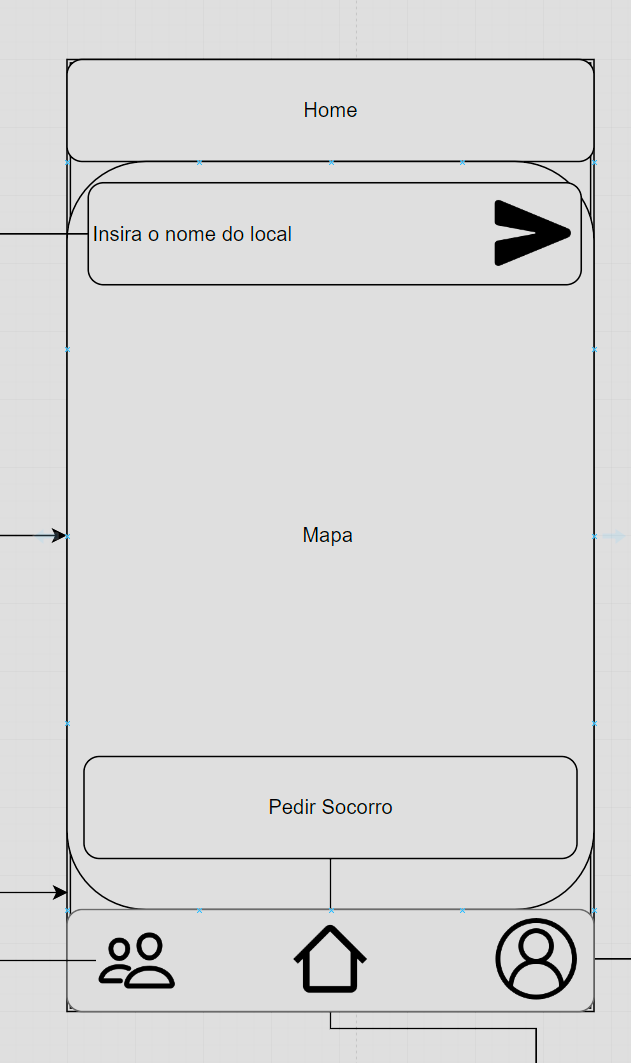
\includegraphics[width=0.5\linewidth]{images/wire-tela-home.png}\\
  \end{center}
  \caption[Wireframe Tela Home]{Wireframe Tela Home}
  \label{fig:wireframe-tela-home}
  \legend{Fonte: Próprio Autor}
\end{figure}
\clearpage
\begin{alineas}
  \item Tipo de interface e interação
  
  Na tela home será utilizada o tipo de tela de interface gráfica onde o usuário irá visualizar sua localização atual no mapa e um campo de busca e um botão de pedido de socorro. A forma de interação será através de toque nos botões tanto da bottom bar quanto do pedir socorro. E através de formulário no campo para inserir o nome do local a ser buscado.
  \item Metáforas
  
  A BottomBar contém ícones os quais remetem as funcionalidades do aplicativo. O ícone com dois bonecos remete a uma lista de contatos. O ícone da casa remete a tela principal de qualquer aplicativo. Já o ícone circular com boneco dentro remete ao perfil em qualquer aplicação. A própria BottomBar já remete a ideia de que é possível navegar entre essas três telas sem que tenha que sair deste menu em si. 
  \item Aprendizibilidade
  
  Previsibilidade – Ao clicar em qualquer um dos ícones da bottom bar o usuário será navegado para a tela correspondente ao ícone.
   
Capacidade de sintetização – O usuário receberá um alert em formato de notificação Toast ao clicar em enviar pedido de socorro e confirmar (caso a confirmação de envio esteja ativada) que deseja enviar.

Familiaridade – Não se aplica.

Consistência – A bottom bar será apresentada sempre no fim das três telas principais (contatos, home e perfil). E os seus ícones estarão sempre na mesma ordem de posição.

Generalização – Não se aplica.
  \item Flexibilidade
  
  Iniciativa de diálogo – É possível cancelar o pedido de socorro ao clicar em cancelar (caso a confirmação de envio esteja ativada).
  
 Multitarefa – Não se aplica.
 
Migração de atividades – Não se aplica.

Substitutividade – Não se aplica.

Personalização – Não se aplica.
  \item Robustez
  
  Observabilidade – O mapa indicará a localização atual do usuário na tela home.
  
Recuperabilidade – O sistema irá emitir um alert em formato de Toast indicando quando houver falha no envio de um pedido de socorro e pedirá para que o usuário refaça a solicitação.

Capacidade de resposta – Ao enviar ou confirmar um pedido de socorro o sistema irá emitir um alerta em formato de Toast indicando que o pedido foi enviado.

Conformidade de realização de atividades – O usuário irá receber na tela um aviso em caso de perda de conexão e pedirá que o usuário se reconecte antes de continuar as operações. 
\end{alineas}

\subsection{Tela 2 - Local}
\begin{figure}[h]
  \begin{center}
  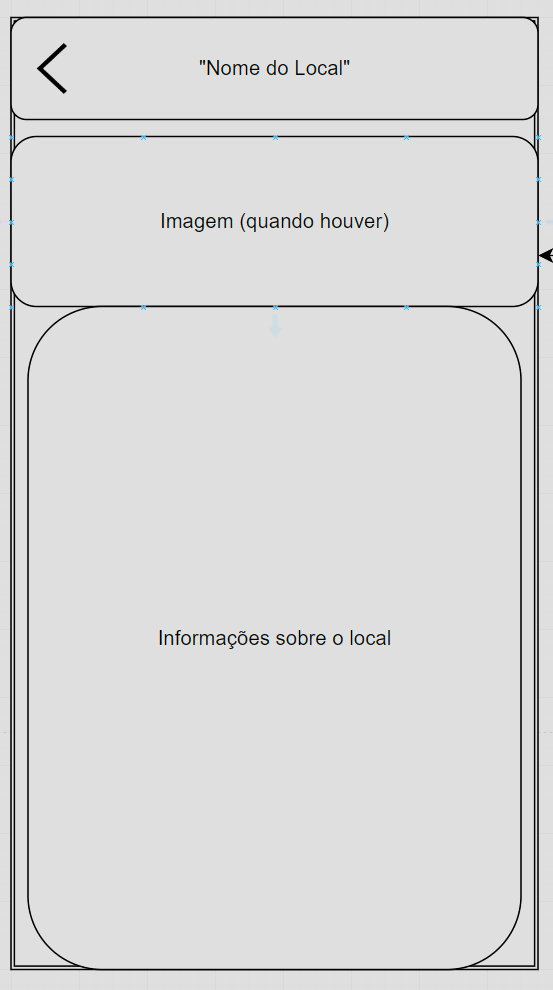
\includegraphics[width=0.5\linewidth]{images/wire-tela-local.png}\\
  \end{center}
  \caption[Wireframe Tela Local]{Wireframe Tela Local}
  \label{fig:wireframe-tela-local}
  \legend{Fonte: Próprio Autor}
\end{figure}
\clearpage
\begin{alineas}
  \item Tipo de interface e interação
  
Na tela lugar será utilizada o tipo de tela de interface gráfica onde o usuário irá visualizar informações sobre o local que ele clicou na tela home. A forma de interação será através de toque no botão de voltar para retroceder a tela home. 
  \item Metáforas
  
Ícone de seta para esquerda indicando a ação de voltar na tela. O ícone estará presente no toolbar da tela no canto superior esquerdo como é de costume em aplicações mobile.
  \item Aprendizibilidade
  
Previsibilidade – Ao clicar no ícone da seta para esquerda espera-se que retroceda uma tela.

Capacidade de sintetização – Não se aplica.

Familiaridade – Não se aplica.

Consistência – O ícone de voltar aparecerá sempre no mesmo local, ou seja, canto superior esquerdo.

Generalização – Não se aplica.

  \item Flexibilidade
  
Iniciativa de diálogo – Não se aplica.

Multitarefa – Não se aplica.

Substitutividade – Não se aplica.

Personalização – Não se aplica.


  \item Robustez
  
 Observabilidade – Os dados apresentados na tela serão do local escolhido na busca na tela anterior.
 
Recuperabilidade – O sistema irá emitir um alert em formato de Toast indicando quando houver falha no envio de um pedido de socorro e pedirá para que o usuário refaça a solicitação.

Capacidade de resposta – Não se aplica.

Conformidade de realização de atividades – Não se aplica. 
\end{alineas}

\subsection{Tela 3 - Perfil}
\begin{figure}[h]
  \begin{center}
  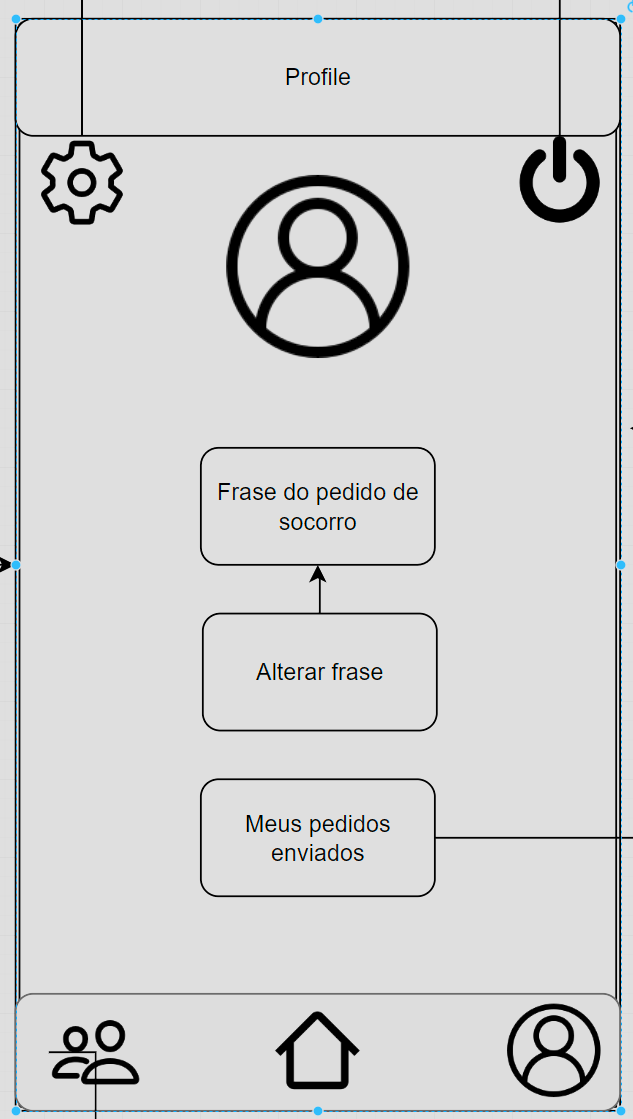
\includegraphics[width=0.7\linewidth]{images/wire-tela-perfil.png}\\
  \end{center}
  \caption[Wireframe Tela Perfil]{Wireframe Tela Perfil}
  \label{fig:wireframe-tela-perfil}
  \legend{Fonte: Próprio Autor}
\end{figure}
\clearpage
\begin{alineas}
  \item Tipo de interface e interação
  
Na tela de perfil será utilizada o tipo de tela de interface gráfica com multi toque. A forma de interação será através de multi toque, onde ao clicar nas opções disponíveis na tela será possível realizar a ação correspondente. 
  \item Metáforas
  
A BottomBar contém ícones os quais remetem as funcionalidades do aplicativo. O ícone com dois bonecos remete a uma lista de contatos. O ícone da casa remete a tela principal de qualquer aplicativo. Já o ícone circular com boneco dentro remete ao perfil em qualquer aplicação. A própria BottomBar já remete a ideia de que é possível navegar entre essas três telas sem que tenha que sair deste menu em si. Há também dois botões de ícones que indicam configurações(engrenagem) e logoff(power).
  \item Aprendizibilidade
  
Previsibilidade – Ao alterar a mensagem do pedido de socorro o usuário recebe um alert em forma de Toast indicando que a alteração foi concluída com sucesso. 

Capacidade de sintetização – Após alterar a mensagem de pedido de socorro a nova mensagem é automaticamente exibida na área da tela onde a mensagem é mostrada.

Familiaridade – Não se aplica.

Consistência – Após a alteração da mensagem de pedido de socorro, os novos pedidos enviados devem ser emitidos com a nova mensagem. Não há alterações para os pedidos já enviados anteriormente.

Generalização – Não se aplica.

  \item Flexibilidade
  
Iniciativa de diálogo – Não se aplica.

Multitarefa – Não se aplica.

Migração de atividades – Caso o usuário altere a mensagem e não clique em salvar, ao sair do foco do campo de inserir a mensagem, o conteúdo atual é salvo como nova mensagem.

Substitutividade – Não se aplica.

  \item Robustez
  
Observabilidade – O usuário irá ver automaticamente a nova mensagem de pedido de socorro assim que ele salvar a sua edição.

Recuperabilidade – Não se aplica.

Capacidade de resposta – Não se aplica.

Conformidade de realização de atividades – Não se aplica

\end{alineas}
\subsection{Tela 4 - Configurações}
\begin{figure}[h]
  \begin{center}
  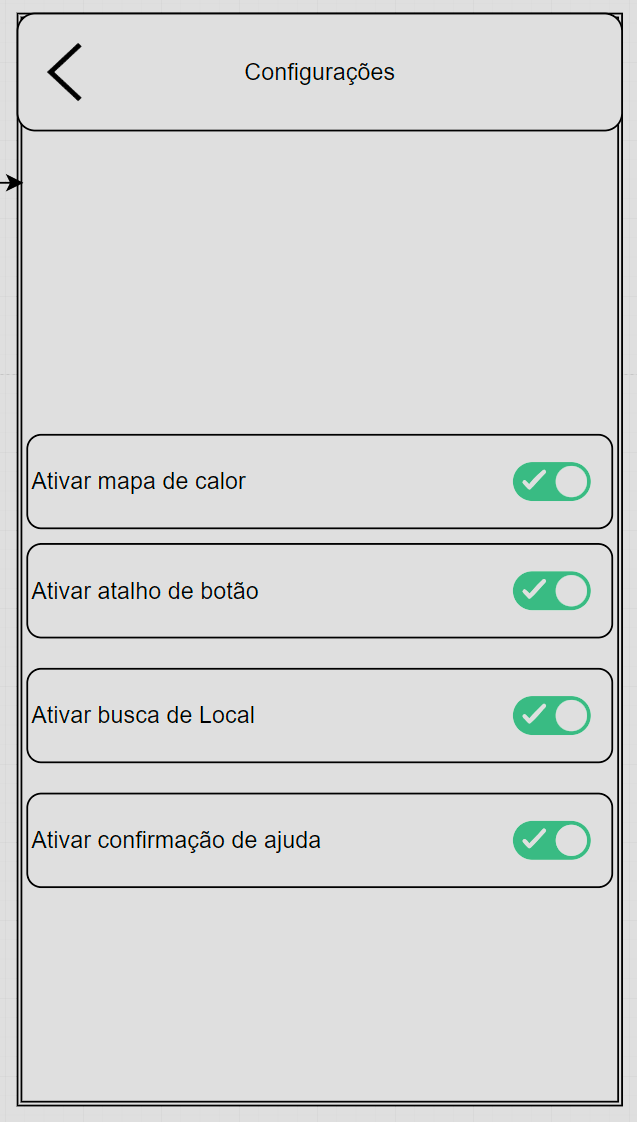
\includegraphics[width=0.7\linewidth]{images/wire-tela-configuracoes.png}\\
  \end{center}
  \caption[Wireframe Tela Configurações]{Wireframe Tela Configurações}
  \label{fig:wireframe-tela-configuracoes}
  \legend{Fonte: Próprio Autor}
\end{figure}
\clearpage
\begin{alineas}
  \item Tipo de interface e interação
  
O tipo de interface será de central de controle, onde o usuário será capaz de ativar ou desativar alguns recursos e configurações do aplicativo. 
A interação será através de gesto de deslize para ativar ou desativar as chaves para cada configuração presente na tela.

  \item Metáforas
  
Os toggles dão ideia de um interruptor para desligar ou ligar a configuração respectiva.
  \item Aprendizibilidade
  
Previsibilidade – Ao acionar o toggle o sistema emitirá alertas de que a respectiva funcionalidade foi liga ou desligada.

Capacidade de sintetização – Não se aplica.

Familiaridade – Os toggle remetem ao interruptor da vida real. 

Consistência – Não se aplica.

Generalização – Não se aplica.

  \item Flexibilidade
  
Iniciativa de diálogo – Não se aplica.

Multitarefa – Não se aplica.

Migração de atividades – Não se aplica.

Substitutividade – Não se aplica.

Personalização – Não se aplica.

  \item Robustez
  
Observabilidade – Ao acionar o toggle de alguma das funcionalidades o usuário será capaz de ver imediatamente o novo estado desta funcionalidade, se está ativada ou não.

Recuperabilidade – Não se aplica.

Capacidade de resposta – Um alert em formato Toast será exibido cada vez em que o estado de uma das funcionalidades for alterado entre liga e desliga.

Conformidade de realização de atividades – Não se aplica
\end{alineas}

\subsection{Tela 5 - Tela Cadastro contato seguro}
\begin{figure}[h]
  \begin{center}
  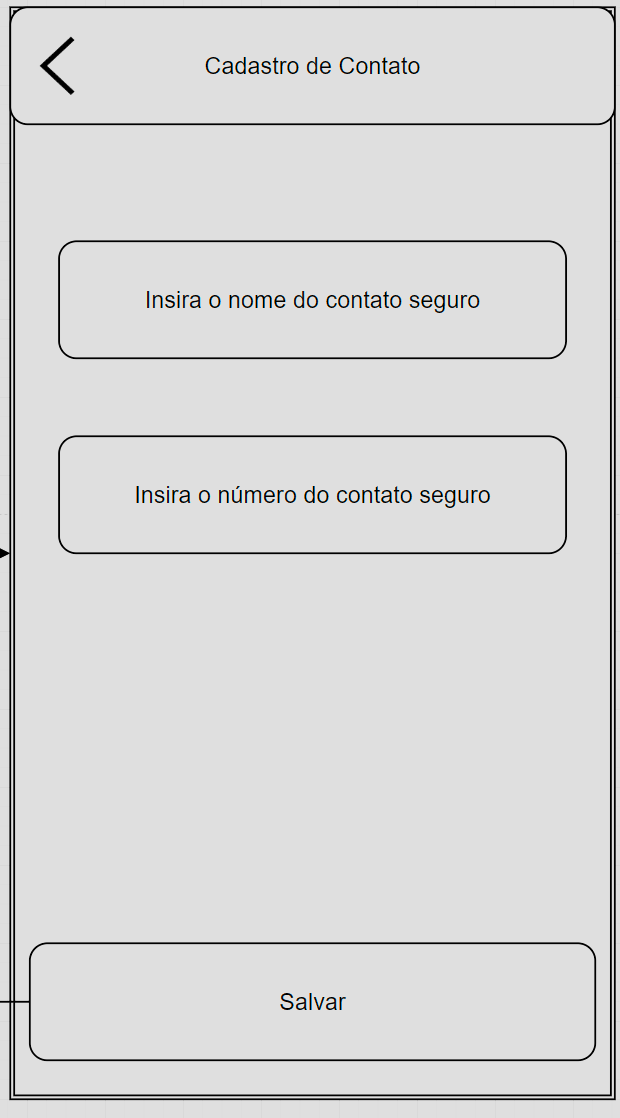
\includegraphics[width=0.7\linewidth]{images/wire-tela-cadsatro-contato-seguro.png}\\
  \end{center}
  \caption[Wireframe Tela Cadastro contato seguro]{Wireframe Tela Cadastro contato seguro}
  \label{fig:wireframe-tela-cadastro-contato-seguro}
  \legend{Fonte: Próprio Autor}
\end{figure}
\clearpage
\begin{alineas}
  \item Tipo de interface e interação
  
A interface será do tipo formulário onde o usuário deverá preencher os dados para cadastro do contato seguro. O tipo de interação será através de preenchimento de campos.
  \item Metáforas
  
Um botão com ícone de seta para esquerda será exibido na app bar indicando a ação de voltar para tela anterior.
  \item Aprendizibilidade
  
Previsibilidade – Um alert em forma de Toast será exibido ao salvar com sucesso um contato.

Capacidade de sintetização – Ao salvar o novo contato com sucesso a tela de listagem de contatos deverá exibir a listagem já com o novo contato inserido na tela. 

Familiaridade – O contato seguro remete a um contato de telefone na agenda do usuário.

Consistência – Não se aplica.

Generalização – Não se aplica
  \item Flexibilidade
  
Iniciativa de diálogo – Não se aplica.

Multitarefa – Não se aplica.

Migração de atividades – Não se aplica.

Substitutividade – Não se aplica.

Personalização – Não se aplica.
  \item Robustez
  
Observabilidade – Não se aplica.

Recuperabilidade – Caso não consiga realizar o cadastro o sistema emitirá um alert em formato de Toast pedindo para o que o usuário refaça a operação.
 
Capacidade de resposta – Será emitido um alerta em formato de Toast informando ao usuário o cadastro no novo contato seguro.

Conformidade de realização de atividades – Ao tentar salvar um novo contato seguro com dados inválidos, por exemplo nome e número de telefone em branco, o usuário receberá uma notificação no campo referido para que faça a correção dele. O mesmo acontecerá caso ele tente adicionar um contato que já esteja salvo na sua lista de contatos seguros. 

\end{alineas}

\subsection{Tela 6 - Tela Listagem de contatos}
\begin{figure}[h]
  \begin{center}
  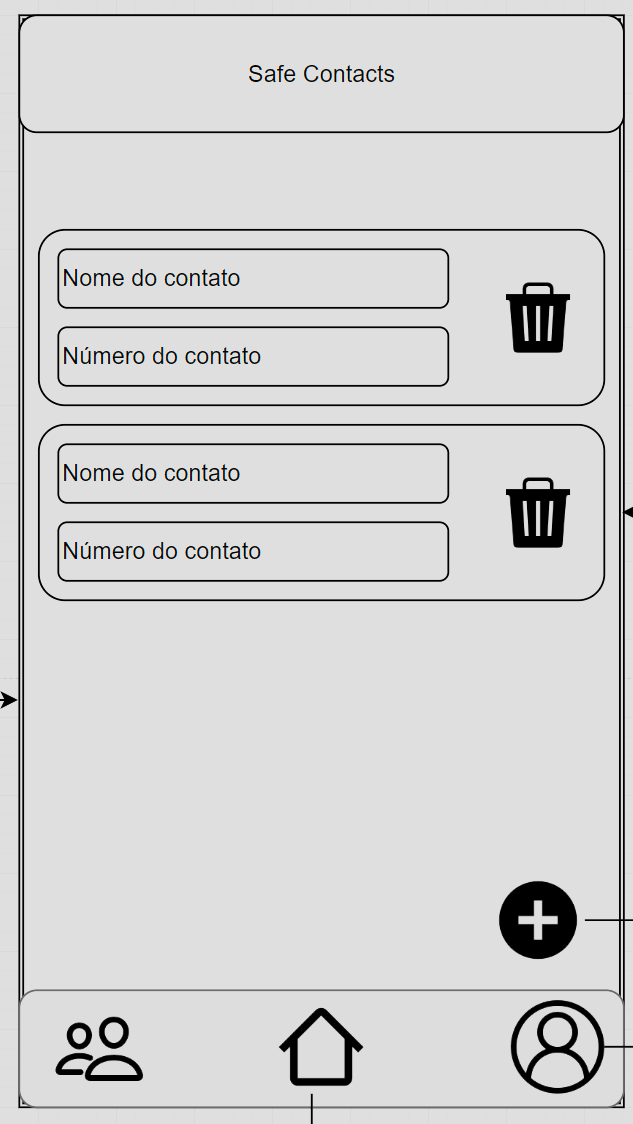
\includegraphics[width=0.7\linewidth]{images/wire-tela-listagem-contatos.png}\\
  \end{center}
  \caption[Wireframe Tela Listagem de contatos]{Wireframe Tela Listagem de contatos}
  \label{fig:wireframe-tela-listagem-contatos}
  \legend{Fonte: Próprio Autor}
\end{figure}
\clearpage
\begin{alineas}
  \item Tipo de interface e interação
  
O tipo de interface utilização será de interface gráfica com listagem. A interação será feita através de gesto de rolagem na tela e com clique para ações. 
  \item Metáforas
  
A BottomBar contém ícones os quais remetem as funcionalidades do aplicativo. O ícone com dois bonecos remete a uma lista de contatos. O ícone da casa remete a tela principal de qualquer aplicativo. Já o ícone circular com boneco dentro remete ao perfil em qualquer aplicação. 

A própria BottomBar já remete a ideia de que é possível navegar entre essas três telas sem que tenha que sair deste menu em si.
O ícone de lixeira será utilizado em cada card de contato indicando que ao clicar ali será executada a ação de deleção do contato seguro correspondente.

  \item Aprendizibilidade
  
Previsibilidade – Ao clicar na lixeira de um determinado contato seguro o usuário receberá um alert em forma de Toast indicando que o contato seguro foi deletado.

Capacidade de sintetização – Ao excluir um contato seguro com sucesso a tela de listagem de contatos é atualizada para retirar o contato seguro que foi removido.

Familiaridade – Não se aplica.

Consistência – Não se aplica. 

Generalização – Não se aplica.

  \item Flexibilidade
  
Iniciativa de diálogo – Não se aplica.

Multitarefa – Não se aplica.

Migração de atividade – Não se aplica.

 Substitutividade – Não se aplica.
 
Personalização – Não se aplica.

  \item Robustez
  
Observabilidade – Ao excluir um contato com sucesso o estado da tela de listagem é atualizado com a nova lista sem o contato que foi deletado.

Recuperabilidade – O contato somente é deixado de ser exibido caso tenha ocorrido com sucesso a deleção. Em caso de insucesso é exibido um alerta em formato de Toast para o usuário indicando para que ele refaça a operação.

Capacidade de resposta – Será exibido para o usuário um alerta em formato Toast indicando a deleção do contato seguro.

Conformidade de realização de atividades – Não se aplica
\end{alineas}

\subsection{Tela 7 - Tela Pedidos de ajuda enviados}
\begin{figure}[h]
  \begin{center}
  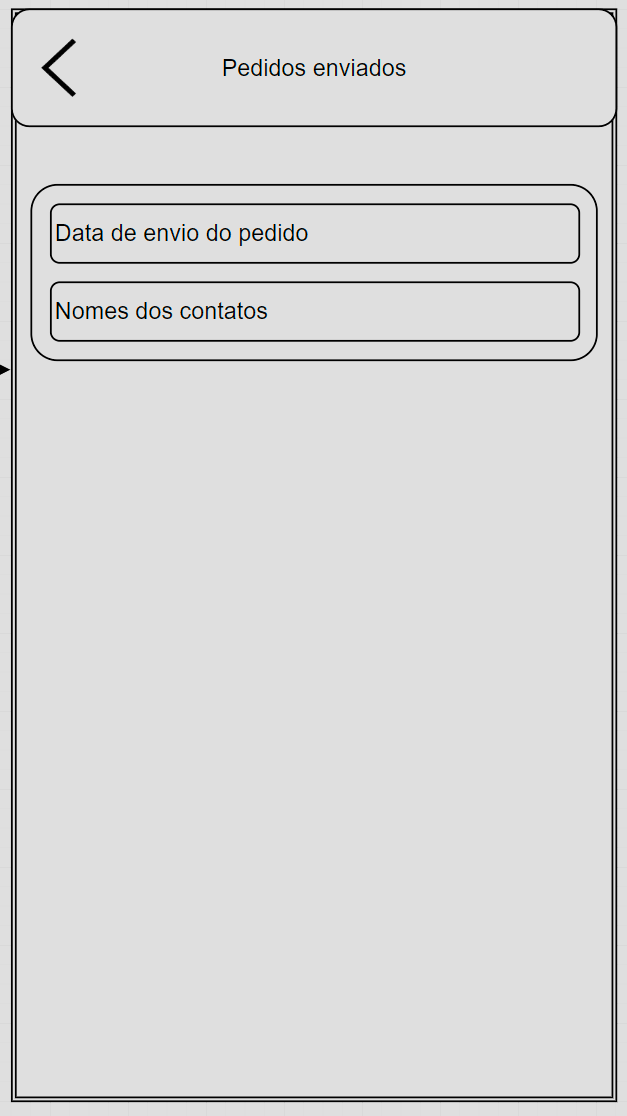
\includegraphics[width=0.7\linewidth]{images/wire-tela-pedidos-enviados.png}\\
  \end{center}
  \caption[Wireframe Tela Pedidos de ajuda enviados]{Wireframe Tela Pedidos de ajuda enviados}
  \label{fig:wireframe-tela-pedidos-ajuda}
  \legend{Fonte: Próprio Autor}
\end{figure}
\clearpage
\begin{alineas}
  \item Tipo de interface e interação
  
Será utilizada nessa tela o tipo de interface de listagem. A interação será através de scroll na tela. 
  \item Metáforas
  
Botão com ícone de seta para esquerda será exibido no canto superior esquerdo da AppBar indicando que irá retornar para tela anterior.
  \item Aprendizibilidade
  
Previsibilidade – Não se aplica.

Capacidade de sintetização – Não se aplica

Familiaridade – Não se aplica.

Consistência – Não se aplica.

Generalização – Não se aplica.
  \item Flexibilidade
  
Iniciativa de diálogo – Não se aplica.

Multitarefa – Não se aplica.

Migração de atividade – Não se aplica.

Substitutividade – Não se aplica.

Personalização – Não se aplica.

  \item Robustez
  
Observabilidade – Não se aplica.

Recuperabilidade – Ao obter erro na busca dos pedidos de socorro enviado do usuário, será emitido um alerta em forma de Toast indicando o erro e pedindo para que ele saia e entre novamente na tela de listagem. 

Capacidade de resposta – Indicar ao usuário quando não houver dados na listagem para serem exibidos.

Conformidade de realização de atividades – Não se aplica.

\end{alineas}


\section{Avaliação de Usabilidade}
\subsection{Rápido e Rasteiro}
As respostas dos usuários podem ser vistas no Anexo A deste documento.

\subsection{Avaliação Heurística}
As respostas dos avaliadores especialistas podem ser vistas no Anexo A deste documento.

\subsection{Correções e melhorias}
O protótipo se mostrou muito agradável aos participantes das avaliações. Alguns foram elencados e serão trabalhados para que sejam feitas as alterações. Alguns pontos foram bastante mencionados e são elencados abaixo.
\begin{itemize}
\item Alteração de contato – Será adicionado um botão ou menu de contexto com apresentará a opção de edição do contato já salvo para que não seja preciso excluir um contato primeiro para depois adicionar seu novo número.
\item Exclusão de contato – Será adicionada uma confirmação para prevenir de uma exclusão de contato acidental.
\item Configurações – Será alterado o título da tela de configurações para corresponder com a tela.
\item Ícone de logout – Será buscado um novo ícone ou repaginado o ícone atual para ficar mais intuitivo. 
\item Alteração de mensagem padrão – Será adicionado um feedback após realizar a alteração da mensagem para que fique mais claro de que a ação ocorreu com sucesso.
\item Campo de busca – Será adicionado um hint ao campo de busca informando o que o usuário deve preencher.
\item Botões de voltar – Diminuição dos ícones de voltar nas telas que possuem.
\end{itemize}
 
\subsection{Nova heurística}
Uma nova heurística a ser introduzida para interfaces mobile acredito que possa ser a opção de login com redes sociais. Hoje em dia é sim muito comum já termos essa opção nos aplicativos, porém ainda existem aqueles que não possuem essa funcionalidade. Essa heurística poderia avaliar a possibilidade de se colocar esse tipo de login, ou seja, se é viável ou se não se aplica dependendo do tipo de sistema.

\section{Conclusões sobre as avaliações}
Após recebidas e analisadas as avalições foi possível perceber que o protótipo se mostra muito promissor. Apesar de poucos apontamentos alguns deles se tornaram bastante perceptíveis visto que mais de um avaliador comentou sobre o mesmo problema. 

Pontos de acessibilidade a serem ajustados
\begin{itemize}
\item Alteração do nome da Tela 7 para condizer e identificar unicamente a tela de configurações
\item Criação de tooltip para cada menu de ação na tela 6 para assim melhor informar o que cada menu faz
\item Atentar ao uso do mapa na codificação para garantia de permissões necessárias.
\item Aplicar hint ao campo de busca para melhor definição do que se espera como entrada
\item Adicionar tolltip ao botão de adicionar contato seguro para melhor acessibilidade
\item Melhorar a formatação dos rótulos dos campos do formulário de cadastro de contato
\item Aplicação de visual de link na listagem de pedidos enviados na tela 8
\item Reavaliar o contraste dos botões dos dialogs
\end{itemize}

